\section{Pregunta N$^{\circ}$1\qquad Andre Gilmer Santos Felix}

\begin{frame}
    \begin{enumerate}\setcounter{enumi}{0}
        \item

              Calcule la curvatura de la gráfica del polinomio de
              $B^{3}_{5}$.
    \end{enumerate}

    \begin{solution}
        La gráfica de una función $y=f\left(x\right)$ es un caso
        especial de una curva parametrizada, de la forma
        \begin{equation*}
            \begin{cases}
                x & =t               \\
                y & =f\left(t\right)
            \end{cases}
        \end{equation*}
        la curvatura viene dada por
        \begin{equation*}
            \kappa=
            \dfrac{
                y^{\prime\prime}
            }{
                {\left(1+{y^{\prime}}^{2}\right)}^{\frac{3}{2}}
            }.
        \end{equation*}

        \begin{figure}[ht!]
            \centering
            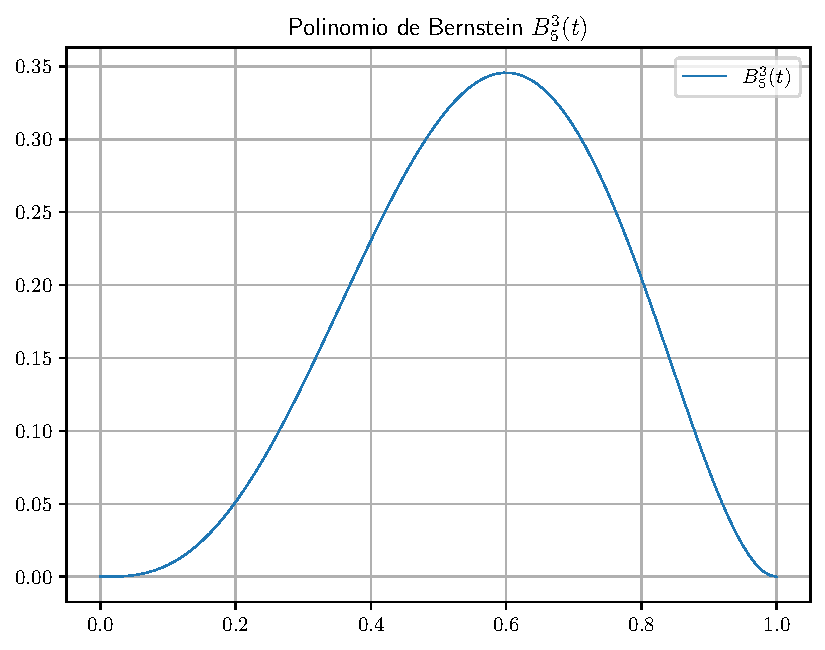
\includegraphics[width=.4\paperwidth]{p1}
        \end{figure}
    \end{solution}
\end{frame}

\begin{frame}
    \begin{solution}
        .
    \end{solution}
\end{frame}